\chapter{Применение обучения с подкреплением для распределения радиоресурсов в гетерогенных сетях малых станций} \label{chapt2}

\section{Общее описание предметной области} \label{sect2_1}

Растущий спрос на поддержание высокого качества услуг беспроводных сотовых технологий создает реальную проблему для телекоммуникационных сетей новых поколений~\cite{TS36.300}. Одним из основных технических требований, предъявляемых к современным сотовым системам, является максимизация фактора повторного использования частот ~\cite{M.1645}. Дефицит лицензированного спектра безусловно приводит к перекрытию диапазонов частот и интерференции между сотами (Inter-Cell Interference, ICI). В сфере контроля и ликвидации интерференции осуществляется интенсивная научная деятельность. В промышленности эти усилия в основном отражаются в виде строгого статического разделения частот или реактивного (в отличие от активного) ручного управления доступным спектром.

Концепция малых сот считается одним из самых практичных способов увеличения общей пропускной способности системы. В этом подходе большое количество маломощных устройств (малые соты) используется для увеличения повторного пространственного использования частот и улучшения местного покрытия. Согласно определению консорциума Small Cell Forum, «малые соты — это управляемые оператором маломощные беспроводные точки доступа с интеллектуальным обслуживанием, работающие в лицензированном диапазоне радиочастотного спектра. К типам малых сот относятся фемтосоты, пикосоты, метросоты и микросоты. Размер сот увеличивается от фемтосот (наименьший) до микросот (наибольший)»~\cite{6171992}. Довольно часто малые соты развертываются без или с небольшим объемом радиопланирования от оператора сети. Для того, чтобы гарантировать в этом случае некоторый заданный уровень качества обслуживания, необходимо внедрять интеллектуальные механизмы управления радиоресурсами для малых сот. Эта концепция принципиально изменяет требования к работе системы сотовых сетей выбиваясь из традиционных представлений о структуре сетей сотовой связи ~\cite{6211486}. При использовании этого подхода большое количество маломощных устройств разворачивается с целью увеличения коэффициента повторного использования частот на выделенной области покрытия. В дополнение к обширному уплотнению, устройства теперь могут часто включаться и выключаться, что вызывает частые неконтролируемые изменения в структуре сети. Таким образом, применение традиционные подходов к контролю интерференции перестало быть возможным, поскольку они основаны на предположении о равномерном гексагональном построении сети и подходят только для централизованного управления базовыми станциями.

Вместе с ростом числа устройств увеличивается количество накладных расходов на передачу управляющей информации. В таких условиях использование централизованных решений становится гораздо менее эффективным, а распределенные алгоритмы для управления ресурсами являются более перспективными. Эффективное управление радиоресурсами и координация интерференции являются неотъемлимыми механизмами для успешного внедрения гетерогенных сетей с малыми сотами.   

В этой главе мы предлагаем подход к управлению передачами на базовых станциях, динамическую схему распределения ресурсов с распределенной двухуровневой процедурой обучения. Мы предполагаем использование только локальной информации с ограничением обмена информацией между соседними сотами. По замыслу, на каждой соте должен быть выработан уникальный набор правил распределения ресурсов, позволяюший всей системе оперативно прийти к оптимальной конфигурации. Мы иллюстрируем применение этой стратегии обучения для задачи выделения частотных поддиапазонов. Каждый обучаемый агент исследует окружающую среду, изучая реакции от конкурирующих агентов и невзаимодействующих базовых макро станций. Полученная информация затем используются, чтобы выбрать наиболее подходящее расписание передач. 

Предлагается рассмотреть распределенную мультиагентную стратегию, где малые соты локально контролируют использование ресурсов для максимизации общей пропускной способности системы. Основная идея заключается в том, чтобы возложить на каждую базовую станцию принятие решение об использовании радиоресурсов. При принятии решения должна учитываться занятость ресурсов окружающих сот. Основной вклад данной работы заключается в следующем. Предложен новый метод для координации интерференции в плотных гетерогенных сетях. Рассмотрены две типичные проблемы часто возникающие в параллельных схемах обучения - разрастание обучаемой модели и блокирование возможности обследования. Предложенный алгоритм осуществляет мониторинг местного уровня интерференции, использование ресурсов и выделяет блоки физических ресурсов оптимальным образом. Алгоритм является полностью распределенным, предполагается отсутствие связи между сотами. Алгоритм быстро адаптируется к изменению интерференции и внешних условий сети, что делает его очень практичным. Дополнительно изучается вопрос о скорости сходимости распределенного механизма и предлагается ряд промежуточных процедур для повышения эффективности обучения. Сходимость и быстродействие алгоритма исследуется путем имитационного моделирования. Результаты предложенного метода оцениваются при помощи моделирования для сети базовых станций LTE и сравниваются с рядом традиционных схем распределения ресурсов. Результаты моделирования на системном уровне показывают, что она обеспечивает значительное улучшение производительности системы для разнородного внедрения с невзаимодействующими агентами без ущерба для эффективности системы в целом.

\section{Описание технологии радиодоступа} \label{section2_2}


\subsection{Архитектура базовой станции} 
Ключевым элементом сети LTE, отвечающим за эффективное использование частотного спектра, является базовая станция. В данном разделе представлена архитектура базовой станции и рассмотрены компоненты, участвующие в процессе управления ресурсами.

\begin{figure}
  \center
  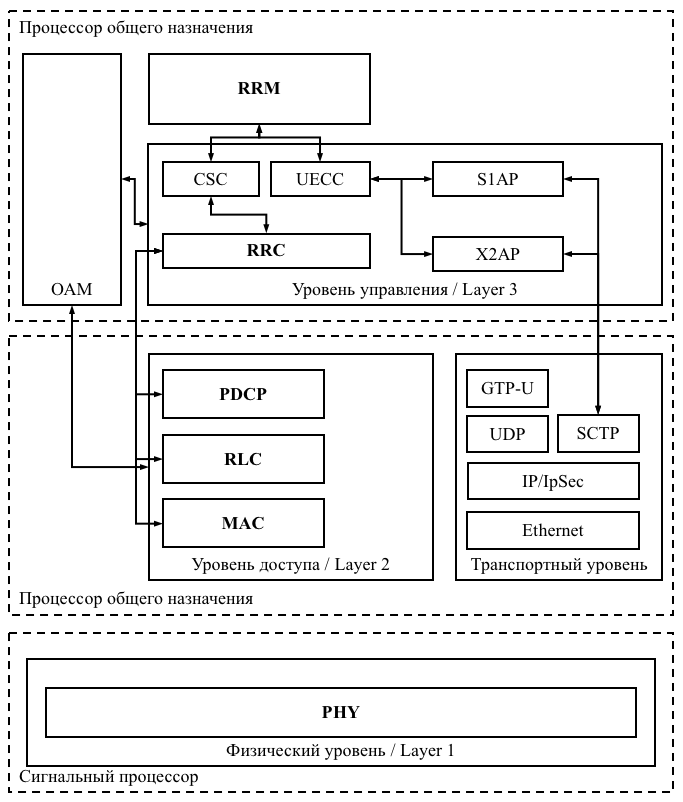
\includegraphics [width=\textwidth]{image7}
  \caption{Архитектура базовой станции LTE. Источник \cite{Aricent}} 
  \label{img:image7}  
\end{figure}


Протокол PDCP (Packet Data Convergence Protocol) обеспечивает компрессию заголовков (ROHC), шифрование, сохранение порядка следования пакетов.

Протокол RLC (Radio Link Control) выполняет функции сегментирования, отброса дубликатов и сохранение порядка следования пакетов \cite{access2008and}. RLC функционирует в одном из трех режимов передачи: прозрачный (transparent mode, TM), передача без подтверждения (unacknowledged mode, UM) и передача с подтверждением (acknoledged mode, AM). В режиме AM поддерживаются специальные функции для повторной передачи данных.

Протокол RRC покрывает следующие функциональные области: передача системной информации, управление RRC соединением (RRC connection control). Сюда относятся процедуры создания, изменения и удаления RRC соединения, пейджинг, активацию защиты соединения, контроль ресурсов для передачи пользовательских данных. Также к этой области относится процедура хэндовера (handover) и конфигурация более низких уровней (PDCP, RLC, MAC).

Протокол RRC также осуществляет настройку измерений качества канала и отчетность на стороне пользовательского устройства, включая настройку и активацию периодов измерений (см. раздел \ref{ch_estimation}). Актуальность информации о состоянии канала напрямую влияет на эффективность передачи пользовательских данных.

Задача управления радиоресурсами решается протоколом RRM (Radio Resource Management). Сюда входит динамическое распределение ресурсов в восходящих и нисходящих направлениях, принятие решений о необходимости хэндовера и допуска пользователей к обслуживанию. Блок RRM также отвечает за ограничение использования спектра с целью контроля интерференции между базовыми станциями.

Задача протокола MAC (Media Access Control) заключается в выделении пользователям частотно временных ресурсов и поддержании гарантий качества обслуживания. Блок MAC также осуществляет выбор сигнально-кодовой конструкции, используемой для обслуживания пользователей.

\subsection{Физический уровень LTE} %\label{section5_2}

Обмен между базовой станцией и абонентским устройством осуществляется кадрами (в терминологии LTE – радиокадр) длительностью 10 мс (см. рис. \ref{img:image8}). Стандарт предусматривает две структуры кадров. Одна для случая частотного разделения каналов (Frequency Division Duplex — FDD), другая - для временного (Time Division Duplex — TDD).

В LTE используется OFDM модуляция, хорошо исследованная при разработке систем DVB, Wi-Fi и WiMAX. В стандарте LTE установлен стандартный шаг между поднесущими ∆f = 15 кГц, что соответствует длительности OFDM-символа 66,7 мкс.

Все временные параметры в спецификации LTE привязаны к минимальному временному кванту $T_s   =  1/(2048 ∙ ∆f)$, где ∆f – шаг между поднесущими, стандартно – 15 кГц. Таким образом, длительность радиокадра – $307200 ∙ T_s$. Отметим, что квант времени соответствует тактовой частоте 30,72 МГц, что кратно стандартной в 3G-системах частоте обработки 3,84 МГц (8×3,84 = 30,72) \cite{access2010lte}.

\begin{figure}
  \center
  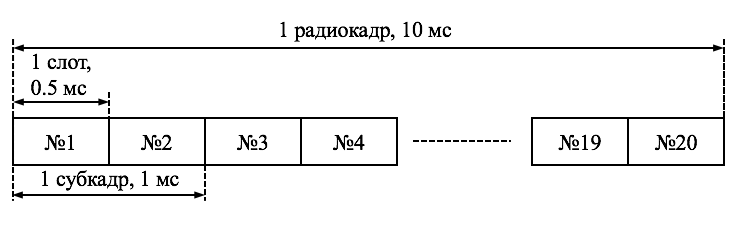
\includegraphics [width=\textwidth]{image8}
  \caption{Структура кадра LTE. Источник \cite{вишневский2009технология}} 
  \label{img:image8}  
\end{figure}


В каждом слоте абонентскому устройству назначается определенный диапазон канальных ресурсов в частотно-временной области – ресурсная сетка (см. рис. \ref{img:image9}). Ячейка ресурсной сетки (ресурсный элемент) соответствует одной поднесущей в частотной области и одному OFDM-символу – во временной. Группа ресурсных элементов образует ресурсный блок. Ресурсный блок – это минимальный квант радиоресурса, выделяемый абонентскому устройству планировщиком базовой станции. Ресурсный блок занимает 12 поднесущих (т.е. 180 кГц) и 7 или 6 OFDM-символов, в зависимости от типа циклического префикса – так, чтобы общая длительность слота составляла 0,5 мс. Число ресурсных блоков в ресурсной сетке зависит от ширины полосы канала и составляет от 6 до 100 (ширина частотных полос восходящего/нисходящего каналов в LTE – от 1,4 до 20 МГц). В новой версии стандарта LTE-A добавлена возможность агрегации до 5 полос шириной 20 МГц \cite{access2013lte}. О распределении ресурсов в каждом слоте базовая станция сообщает в управляющем канале, располагающемся в начале каждого субкадра.

\begin{figure}
  \center
  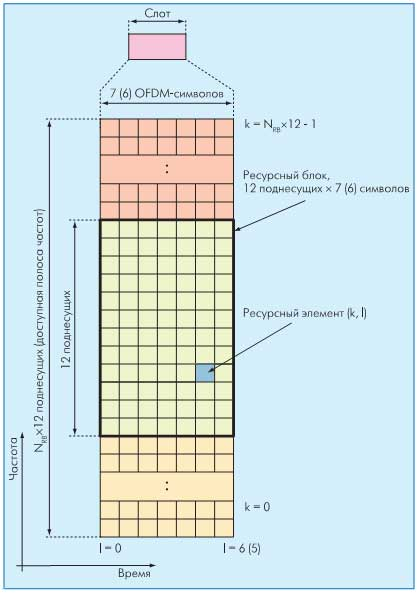
\includegraphics [width=0.9\textwidth]{image9}
  \caption{Ресурсная сетка LTE при стандартном шаге поднесущих ∆f = 15 кГц. Источник \cite{вишневский2009технология}} 
  \label{img:image9}  
\end{figure}

Поднесущие модулируются посредством 4-, 16- и 64-позиционной квадратурной фазово-амплитудной модуляции (QPSK, 16-QAM или 64-QAM). Соответственно, один символ на одной поднесущей содержит 2, 4 или 6 бит информации. При стандартном префиксе символьная скорость составит 14000 символов/с. Сигнал с полосой 20 МГц содержит 100 ресурсных блоков или 1200 поднесущих, что дает общую скорость в канале от 33,6 до 100,8 Мбит/с.

Для повышения надежности передачи на физическом уровне стандарт LTE использует механизм HARQ (Hybrid Automatic Repeat Request). HARQ представляет собой комбинацию высокоскоростного помехоустойчивого кода и стандартного механизма ARQ \cite{access2008and}. Эта технология позволяет пользовательскому устройству запросить дополнительные проверочные биты при обнаружении ошибки декодирования.

\subsection{Оценка канала} \label{ch_estimation}

Для эффективного осуществления передачи данных базовая станция должна иметь оценку качества канала до обслуживаемого пользователя. Эта оценка используется для планирования расписания передач. Стандарт LTE предусматривает возможность запросить у пользователя отчет с оценкой качества канала. Для того чтобы задать формат отчетов о качестве канала, базовая станция посылает пользователю служебное сообщение RRC ConnectionReconfiguration \cite{access2012lte} с указанием следующих параметров:

При получении сообщения RRC ConnectionReconfiguration \cite{access2012lte} пользовательское устройство проводит измерения мощности пилотных сигналов соседних станций и через время равное reportInterval посылает их в отчете Measurement report. Эти величины называются RSRP (Reference Signal Received Power) \cite{access2010lte} и квантуется в соответствии с рисунком 10.

\section{Обзор методов координации интерференции в сотовых сетях}
%\blindtext

В данном разделе представлен обзор смежных работ в области управления радиоресурсами и координации интерференции в сотовых сетях. Существует множество исследований по данной теме, в особенности, на тему интерференции между макростанциями. На данный момент этот эффект является одним из основных сдерживающих факторов в сценариях с плотным развертыванием малых сот. В связи с этим в мире ведутся многочисленные исследовательские работы, посвященные различным вариантом управления ресурсами в разнородных сетях. Подробный обзор основных методов управления интерференцией, совместимых с LTE представлен в ~\cite{cite_overview}.


%NEW SECTION
%======================================================
\subsection{Методы частотного разделения} \label{sect4_1}

За последние 40 лет проблеме повышения производительности сетей сотовой связи было посвящено множество исследовательских работ. В данном разделе представлен общий обзор направлений современных исследований в данной области.

Как правило, среди алгоритмов повторного использования частот выделяют:
\begin{itemize}
\item Полное повторное использование частот (Full Frequency Reuse), когда вся полоса полностью используется каждой сотой независимо от местоположения абонентов. Распределение ресурсных блоков в этом случае осуществляет планировщик базовой станции, а информацию о распределении ресурсов базовая станция сообщает абонентским станциям по специальному управляющему каналу.
\item Жесткое повторное использование частот (Hard Frequency Reuse), когда вся полоса частот разделена на фиксированное количество полос, которые назначаются сотам в соответствии с частотным планом сети (см. рис. \ref{img:image11}).

\begin{figure}[ht] 
  \center
  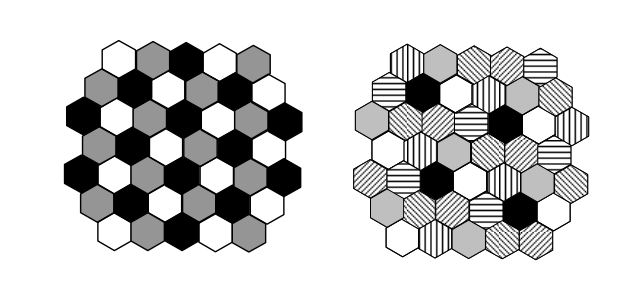
\includegraphics {image11}
  \caption{Схема распределения частотных каналов между сотами ($$N = 3, N = 7$$)} 
  \label{img:image11}  
\end{figure}


\item Мягкое повторное использование частот (Soft Frequency Reuse — SFR), когда площадь, обслуживаемая базовой станцией, разделяется на две зоны — центральную, в которой абонентским устройствам доступны все частотные ресурсы и зону, находящуюся на границе, в которой устройствам доступна только часть ресурсов. Отсутствие частотных ресурсов на границе соты, может привести к существенному уменьшению пропускной способности в канале. Поэтому на частотах, используемых устройствами на границе, повышается мощность передачи, чтобы увеличить отношения SINR, а значит и значение пропускной способности (см. рис. \ref{img:image12}).
\end{itemize}

\begin{figure}[ht] 
  \center
  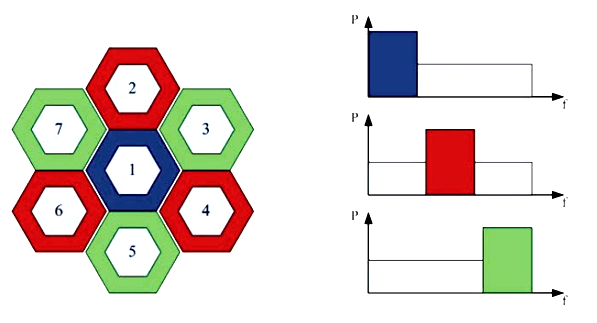
\includegraphics {image12}
  \caption{Схема использования частот и профили мощности для метода SFR} 
  \label{img:image12}  
\end{figure}

Одна из первых статей, описывающих динамическое назначение каналов (Dynamic Channel Allocation — DCA) для сетей с коммутацией каналов была представлена в 1971 году \cite{cox1971dynamic}. Для осуществления вызова устройству на время разговора назначался канал из стека доступных каналов. После завершения разговора, канал возвращается в общий стек. Чтобы избежать помех, канал, который используется в одной соте мог быть назначен одновременно в другую соту, только если расстояние между двумя сотами было больше, чем минимальное расстояние повторного использования.

Помимо DCA, в то же время появилась схема заимствования каналов (Borrowing Channel Assignment — BCA), которая была предложена в работах \cite{engel1973statistically1}, \cite{engel1973statistically2} и \cite{electosvyasru-2017}. В отличие от схемы DCA, где соты могли использовать все каналы, BCA сначала фиксирует каналы, а затем позволяет загруженным сотам заимствовать у соседних сот неиспользуемые каналы. На рисунке \ref{img:image13} показана возможность использования незанятых каналов, доступных белым сотам, серой сотой, указанной стрелкой.

\begin{figure}[ht] 
  \center
  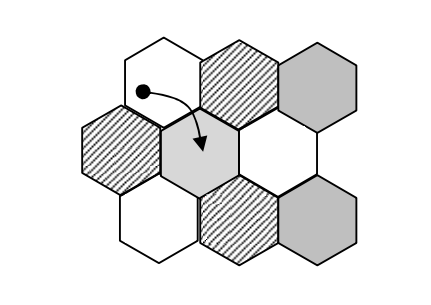
\includegraphics {image13}
  \caption{Схема заимствования каналов BCA. Источник \cite{engel1973statistically1}} 
  \label{img:image13}  
\end{figure}

Отметим, что если динамическое назначение каналов на базовой станции осуществляется независимо от решения соседних базовых станций, то для эффективной борьбы с интерференцией станция должна иметь возможность измерения уровня интерференции в канале передачи.

Для динамической координации интерференции в LTE между базовыми станциями поддерживается сигнализация через специфицированный интерфейс X2 \cite{network2008x2}.

Данный интерфейс позволяет напрямую между станциями обмениваться сообщениями, такими как: индикатор мощности передачи ресурсных блоков RNTP – Relative Narrowband Tx Power, индикатор высокого уровня интерференции HII – High Interference Indicator, и индикатором перегрузки OI – Overload Indicator.

RNTP - двоичный индикатор, каждый бит которого указывает, превышает ли мощность передачи соответствующего частотного блока некоторое пороговое значение. С помощью RNTP базовая станция информирует своих соседей о том, с какой мощностью будут излучаться все частотные блоки на длительности одного или нескольких кадров.

HII - двоичный индикатор, каждый бит которого указывает на предстоящую передачу в определенных частотных блоках в восходящем канале, которая может увеличить уровень интерференции на соответствующих ресурсах.

OI – индикатор, который отражает уровень интерференции (низкий, средний, высокий), на частотных блоках восходящего канала.
Другая техника — Reuse Partitioning. Этот алгоритм является разновидностью статического планирования и нацелен на увеличения пропускной способности путем использования различных методов совместного использования частот для конкретного пользовательского устройства. Впервые этот алгоритм представлен в 1983 году \cite{halpern1983reuse}, под названием Reuse Partitioning. В последствие, в конце 90-x он был заново открыт как Intelligent Underlay-Overlay \cite{ling1996capacity}, \cite{wille1996capacity}, \cite{nielsen1997capacity}, \cite{wigard1997improved}. Сейчас, благодаря работе WiMAX форума и консорциума 3GPP, этот алгоритм известен как алгоритм частичного повторного использования частот, Fractional Frequency Reuse — FFR \cite{wimax2006technical}.

Алгоритм FFR разделяет полосу частот на две группы — внутреннюю и внешнюю. Внутренняя полоса частот назначается для передачи на пониженной мощности устройствам, расположенным близко к обслуживающей базовой станции. Для устройств, находящими на границе соты, выделяется внешняя полоса с коэффициентом повторного использования большим единицы.

В то время как reuse partitioning и intelligent underlay-overlay в большей степени известны как алгоритмы разделения частот в сетях с коммутацией каналов, FFR чаще используется в сетях с пакетной коммутацией.

Обобщение алгоритма FFR было предложено в работах \cite{bonald2005inter}, \cite{bonald2006inter}. Алгоритм работает с произвольными участками внутри соты, в каждом из которых пользовательское устройство обслуживается с определенным профилем передачи (transmission profile). Профиль представляет собой определенной набор активных передатчиков. Аналогичные исследования описаны в работе \cite{liu2006inter}.

Алгоритм динамической локальной координации (dynamic local coordination) представлен в работе \cite{sternad2003attaining}. Данный алгоритм основан на использовании общего планировщика между секторами внутри одной соты и разных коэффициентов повторного использования частот, для устройств, в зависимости от расстояния до обслуживаемой базовой станции. На основе этой работы, в статье \cite{necker2007local}, проведена всесторонняя оценка производительности алгоритмов.

Гибридные и децентрализованные схемы координации интерференции были предложены компанией Alcatel-Lucent в работах \todo{[37-39]} \cite{R1-050407,R4-092042,R1-081873} и оказались особенно эффективны для балансировки нагрузки сот.

Исследователи из Nortel в работах [40], [41] и [42] предлагают адаптивную схему повторного использования частот (Adaptive Fractional Frequency Reuse — AFFR), основанную на подходах FFR и SFR, которая также относится к гибридным децентрализованным схемам координации интерференции. Согласно алгоритму AFFR сота может работать в одном из четырех режимов, которые различаются различными политиками совместного использования частот. Первый режим предполагает передачу на полной мощности во всем доступном частотном диапазоне. В противоположность первому режиму четвертый режим предполагает разделение частотного диапазона на 3 части, аналогично HFR. Режимы 2 и 3 предполагают использование SFR с различными уровнями мощности. В данном алгоритме базовые станции могут взаимодействовать друг с другом и отправлять запросы на использование того или иного режима работы, если уровень интерференции становиться слишком высоким.

Исследователи из Texas Instruments в работах [43], [44] предлагают внести дополнения в подход FFR, так чтобы размер частотных блоков мог адаптивно настраиваться между сотами с помощью специального контроллера. Эта концепция представляет собой гибридную, децентрализованную схему координации интерференции.

Другие примеры распределенных схем представлены в работах \cite{rahman2008interference}\cite{li2006downlink}.

В работах [38] и [39] методы повторного использования частот в сетях с OFDMA анализируются на примере сетей LTE. Результаты моделирования в [39] показывают, что схемы с полным повторным использованием частот обеспечивает наилучший показатель пропускной способности, как для восходящего, так и для нисходящего канала, однако пользователи находящиеся на границе соты (cell edge users) испытывают высокий уровень интерференции и имеют приблизительно одинаковые показатели спектральной эффективности. В работе [38] показано, что спектральная эффективность пользователей, находящихся на границе соты, может быть увеличена с помощью использования схем согласованного частичного использования частот, в которой различные подканалы имеют различные уровни мощности передачи. Увеличение до 20 процентов в совокупной пропускной способности получено для схемы частичного повторного использования.

Математически, задачу назначения частотных диапазонов базовым станциям можно свести к задаче на графах. Алгоритмы, использующие теорию графов, как правило, представляют сеть в виде неориентированного графа, вершины которого обозначают базовые станции, а ребра – наличие интерференции между ними.

Одна из первых работ, авторы которой свели задачу назначения каналов к задаче раскраски графа, была представлена в 1980 году \cite{wimax2006technical}. Ранние работы по моделированию интерференции в сетях, основывались на моделях, использующих особый тип графов — граф единичных кругов \cite{bonald2005inter}, неориентированный граф, узлы которого является центрами единичных окружностей. Если пересечение двух окружностей не пусто, тогда соответствующие узлы соединяются ребром. Характерный вид unit disk graph представлен на рисунке \ref{img:image14}.

\begin{figure}[ht] 
  \center
  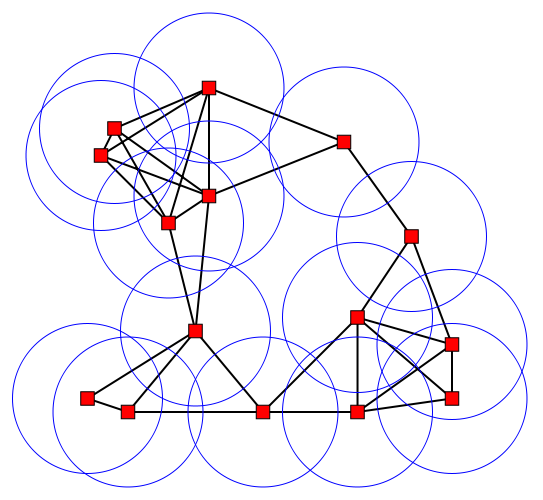
\includegraphics [width=10cm]{image14}
  \caption{Пример графа единичных кругов} 
  \label{img:image14}  
\end{figure}

Краткий обзор алгоритмов раскраски графов описан в работе \cite{bonald2006inter}. Большая часть работы посвящена обзору алгоритмов на гексагональных сетках. Также в работе рассмотрены результаты для unit disk graph. Изучению изменения характеристик сети вследствие ограничений, налагаемых введением честности между пользователями и профилем QoS, отражены в статье \cite{liu2006inter}. Иной подход к построению графов, предлагают работы, в которых вершины интерференционного графа представляют собой пользовательские устройства \cite{sternad2003attaining}.

С появлением децентрализованных сетей с пакетной коммутации в сотовой связи, схемы, основанные на взаимодействии между устройствами, становятся все более популярными. Теория игр исследует такие взаимодействия, поэтому ее методы были использованы для решения задач динамического назначения канальных ресурсов несколькими устройствами в ряде работ [42] и [43].

Другой поход к координации интерференции в сети представляет использование различных профилей мощности (Power Control). Исторически, Power Control использовался в сотовых сетях для решения проблемы, когда пользовательское устройство, находящееся на краю соты оказывается заглушенным устройствами, расположенными рядом с базовой станцией \cite{li2006downlink}, \cite{gilhousen1991capacity}. Это проблема решается ограничением мощности в восходящем канале, при постоянном уровне мощности на базовой станции. Такой подход, хотя и является не оптимальным с точки зрения общей пропускной способности или спектральной эффективности, но обеспечивает честность по отношению к пользователям, находящимся на границе соты.

Последние исследования для сетей 4-го поколения предлагают компромиссный подход, путем частичной компенсации потери мощности сигнала для пользователей находящихся на границе \cite{castellanos2008performance}, в отличие от полной, использовавшейся ранее. Частичная компенсация потери мощности сигнала обеспечивает улучшение общей пропускной способности на 20 процентов по сравнению с традиционными методами, если расстояние между базовыми станциями находится в промежутке от 500 м до 1 км, при ширине канала в 10 МГц. Для сценариев с небольшим межсотовым расстоянием, менее 500 м, частичная компенсация также показывает рост пропускной способности крайних пользователей (5-процентиль) на 10-15 процентов по сравнению с традиционными методами.

%NEW subSECTION
%======================================================
\subsection{Методы согласованной передачи} \label{sect4_2}
Технология MIMO (множественный вход – множественный выход) позволяет значительно увеличить помехоустойчивость каналов связи в условиях многолучевого распространения сигналов [49, 50]. Как правило, под аббревиатурой MIMO подразумевается целый ряд технологий:
\begin{itemize}
\item Использование, так называемых, «интеллектуальных» антенн (intelligent antennas), позволяющих формировать многолучевые диаграммы направленности. Данная технология позволяет увеличить эффективность использования спектра за счет передачи данных в параллельных лучах.
\item Использование пространственно-временного кодирования (Space-Time Coding – STC)
\item Использование поляризационного разделения каналов, поляризационной обработки сигналов.
\end{itemize}

Все разновидности технологии MIMO направлены на достижение одной цели – увеличение пиковой скорости передачи данных за счет увеличения соотношения сигнал/шум на приемном устройстве.

Наиболее широкое распространение получила технологи MIMO на основе пространственно-временного кодирования \cite{oestges2010mimo,3GPPTS2530,3GPPTR25814}, которая вошла в стандарты LTE 3GPP.

Алгоритмы координации интерференции в многоантенных системах были обобщены понятием сетевого MIMO (network MIMO, Net-MIMO, Cooperative MIMO, CO-MIMO или Ad-hoc MIMO), которое предполагает передачу или прием сигнала с помощью многоантенных систем на нескольких базовых станциях \cite{jindal2006mimo}. На нисходящем канале несколько базовых станций могут передавать по нескольким MIMO-путям одному и тому же пользовательском устройству. Аналогично, в восходящем канале сигналы от пользовательского устройства могут быть приняты одной или несколькими базовыми станциями.

\begin{figure}[ht] 
  \center
  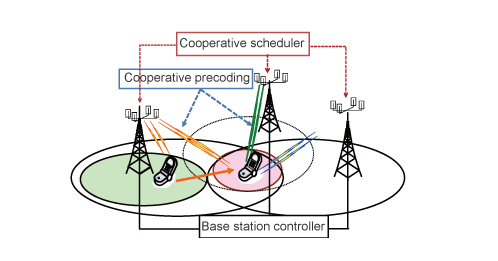
\includegraphics[width=15cm] {image15}
  \caption{Принципиальная схема организации сетевого MIMO} 
  \label{img:image15}  
\end{figure}


Одна из проблем реализации сетевого MIMO является задержка в ходе обмена информацией между базовыми станциями. В стандарте LTE минимальные задержки при обмене информацией между базовыми станциями с помощью интерфейса X2 составляют 20 мс. В то время как планирование ресурсов осуществляется каждую миллисекунду. Поэтому при обработке данных требуется учет этой особенности.

Технология координированной множественной передачи (CoMP) подразумевает обслуживание одного абонентского устройства несколькими базовыми станциями. Координированная передача и прием рассматриваются как способ, с помощью которого можно увеличить скорость передачи абонента, находящегося на границе соты. При этом повышение скорости передачи в нисходящем канале достигается за счет уменьшения уровня интерференции, а в восходящем канале - за счет параллельной обработки принятого сигнала на нескольких базовых станциях[55] .

В нисходящем канале можно выделить 2 основных метода кооперативной многоантенной передачи: совместная обработка (Joint Processing — JP) и координированное планирование (Coordinated Beamforming/Coordinated Scheduling — CB/CS). Оба метода представлены на рисунке \ref{img:image15}. В случае совместной обработки передаваемые данные доступны на всех базовых станциях, с которых ведется передача. Однако существует два различных варианта реализации этого подхода. В первом варианте осуществляется одновременная передача с нескольких базовых станций. А во втором варианте базовая станция, которая осуществляет передачу данных, выбирается динамически. То есть передача осуществляется только с одной базовой станции в каждый момент времени. При этом данные для передачи доступны на нескольких базовых станциях.

В случае координированного планирования передач данные всегда передаются только с одной базовой станции, при этом решение о расписании передач делается с учетом информации о планировании от нескольких соседних базовых станций \cite{karakayali2006network}, \cite{andrews2007overcoming}. При координированном приеме данных (т.е. при восходящей передаче) можно также выделить два различных варианта. Первый вариант — это совместный прием сигнала от пользовательского устройства на нескольких базовых станциях (Joint Reception — JR). Второй вариант - это координированное планирование передач с целью уменьшения или полного погашения интерференции. Кроме этого, возможна комбинация обоих названных вариантов.

%NEW subSECTION
%================================================
\subsection{Формирование диаграммы направленности} \label{sect4_3}
В последнее время, планирование ресурсов с возможностью формирования диаграммы направленности \cite{svedman2007opportunistic} является предметом пристального изучения.

В работе \cite{hu2008radio} исследована производительность системы связи, в которой применяется схема формирования диаграммы направленности антенн с псевдослучайной перестройки лучей (Organaized Beam Hopping — OBH). Сокращение интерференции в схеме OBH достигается путём пространственного разнесения передач от соседних базовых станций. Анализ производительности схемы OBH показал увеличение спектральной эффективности порядка 1 бит/с/Гц. Результаты были получены при помощи моделирования сотовой сети, состоящей из сот радиусом 1 км, каждая из которых имеет шесть лучей. В работах также отмечается ряд нерешенных вопросов, в том числе связанных с механизмом адаптации к различным профилям мобильного трафика.


%NEW subSECTION
%================================================
\subsection{Альтернативные подходы} \label{sect4_4}
Техника подавления помех (Interference Cancellation — IC), предложенная более 20 лет назад, хорошо известна в литературе, посвященной проблеме борьбы с интерференцией в беспроводных сетях. Основная концепция заключается в восстановлении сигналов помех, а затем вычитании их из принятого сигнала. Как правило, это предполагает хранение принятого сигнала в буфере для последующей обработки.

Подавление помех может применяться как на восходящем, так и нисходящем канале, но из-за сложности реализации, оно рассматривается, главным образом, как техника для восходящего канала и реализуется в приемнике базовой станции. Исчерпывающий обзор методов подавления помех, используемых в сотовых сетях, представлен в работе \cite{andrews2005interference}.
Dirty paper and sphere coding — это две последние инновации в алгоритмах кодирования, которые являются потенциально применимыми к сетям 4-го поколения.

Основная концепция Dirty paper coding заключается в предварительном кодировании каждого потока таким образом, что нужный сигнал отображается в некоторое кодовое слово. Приемник, обладающий знаниями о кодовом пространстве, может быть использован для успешного декодирования полезного сигнала в присутствии интерференции с помощью декодера \cite{choi2006capacity}.

Sphere coding еще один метод, которому уделяется большое внимание в качестве подхода для устранения помех. Суть подхода заключается в поиске N-мерной гиперсферы некоторого предопределенного радиуса R в кодовом пространстве. Выбор радиуса представляет собой компромисс между экспоненциально растущей сложностью поиска, с ростом R, и более высокой вероятностью ошибки при меньшем значении радиуса \cite{barbero2007performance}.

\subsection{Перспективные методы частотного разделения}

Для плотных неконтролируемых внедрений базовых станций задача управления интерференцией между сотами является более сложной, чем в традиционных операторских сотовых сетях. Один из перспективных методов управления радиоресурсами основывается на проведении предварительного исследовании радиоокружения, с целью выявления статистических данных об использовании ресурсов. Затем извлеченные данные могут быть использованы для непосредственного принятия решений (как в \cite{mab}) или (как, например, в \cite{q-learning}) для построения оптимальной схемы распределения ресурсов. В частности, в работе~\cite{q-learning} исследуется вопрос о самоорганизации и децентрализованном управлении интерференцией в сети фемтосот с целью разделения радиоресурсов между фемтосотами и макроокружением (сетью макро базовых станций и другими источниками интерференции). В этой работе рассмотрен многоагентный подход к обучению на основе распределенного Q-обучения (Q-learning). Малые соты меняют свою мощность передачи, чтобы максимизировать суммарную выходную мощность, в то время как суммарная интереференция макро пользователей в нисходящей линии связи поддерживается в заданных пределах.

В \cite{mp-qlearning} и \cite{fzq-learning} авторы предлагают другие схемы на основе Q-обучения и демонстрируют значительный выигрыш по сравнению с обычными методами повторного использования частот с точки зрения пропускной способности пользователей сотовой сети. Однако, эти методы устанавливают жесткие требования к качеству канала обратной связи и менее эффективны с точки зрения времени сходимости в динамичных случаях с гибким трафиком. 

В \cite{mab} предложен подход с использованием машинного обучения с подкреплением, где базовые станции автономно выбирают наиболее эффективную схему использования спектральных ресурсов из заранее заданного набора. Это позволяет гибко управлять компромиссом между фазой изучения окружающей среды и фазой использования накопленной информации. Похожие схемы с возможностью автоконфигурации и самооптимизации также были представлены в \cite{local-area}, где алгоритм позволяет сотам динамически выбирать начальные участки спектра и опирается на механизмы контроля мощности. Управление интерференцией между сотами было также изучено в \cite{on-uplink}, где авторы предложили схему планирования с фиксированными вероятностями выбора ресурсных блоков. В данном случае, сложность предлагаемых стохастически схем управления радио ресурсами является относительно низкой, поскольку они предполагают децентрализованный подход и требуют только ограниченный объем передачи управляющей информации. Однако, эти схемы могут быть неэффективными при рассмотрении сетей малых сот большого размера.
Еще один интересный децентрализованный подход был предложен в ~\cite{1666484}, где проблема распределения каналов сводится к задаче раскраски графа. Единственная информация, необходимая алгоритму, - обратная связь по уровню интерференции на выбранном канале. В~\cite{Duffy:2008:CAD:1377038.1377164} и ~\cite{4177619}сложность и скорость сходимости изучены для класса децентрализованных алгоритмов раскраски. Отметим, что проблема, рассматриваемая в данной главе, не может быть сведена к раскраске графа, так как соты могут находиться на одном и том же поддиапазоне, а границы частот поддиапазонов не фиксируются.
В то время как описанные решения обеспечивают подходы к управлению распределением ресурсов, они не учитывают ряд важных моментов, рассматриваемых далее в работе. Предлагается рассмотреть метод управления интерференцией, сделав упор на исследование нескольких ощутимых недостатков мультиагентного обучения. Основной проблемой является рассогласование между состоянием всей системы и поведением каждого агента в отдельности. В перспективе исследования скорости сходимости система имеет два состояния - состояние ''разведки'', где изучение окружающей среды движет систему к стабильному состоянию, и состояние ''эксплуатации'' - стабильное состояние, где эффективность обучения низка в связи с необходимостью сохранить стабильность системы. Недостатком такого подхода является то, что система интенсивно изучает среду в одном состоянии (где поведение агентов определяется, главным образом, исследованием поведения окружения), а затем работает в другом состоянии (определяемым эксплуатационным поведением агентов). В этой главе мы предлагаем первоначально заставить группу агентов вести себя уникальным образом, чтобы добавить больше смысла в процесс обучения. Мы также изучаем еще одну проблему схемы обучения, которая заключается в разрастании пространства состояний обучаемой модели с увеличением количества поддиапазонов.
Цель этого исследования заключается в получении схемы управления интерференцией посредством распределения частотных ресурсов с применением нескольких новых усовершенствований поведения обучаемых агентов с акцентом на их сосуществовании в плотной сотовой сети.


\section{Постановка задачи распределения ресурсов}
\subsection{Архитектура системы}
В этой главе мы рассматриваем сотовые сети технологии LTE/LTE-А с разнородным внедрением базовых станций, таких как макросоты и малые соты, как показано на Рис.~\ref{fig:architecture}. Малые соты обычно используются для улучшения покрытия в помещениях и для повышения общей пропускной способности в густонаселенных районах. Основной упор в данном разделе сделан на сосуществование малых сот с макросредой и некооперативными группами малых сот.

\begin{figure}
    \centering
    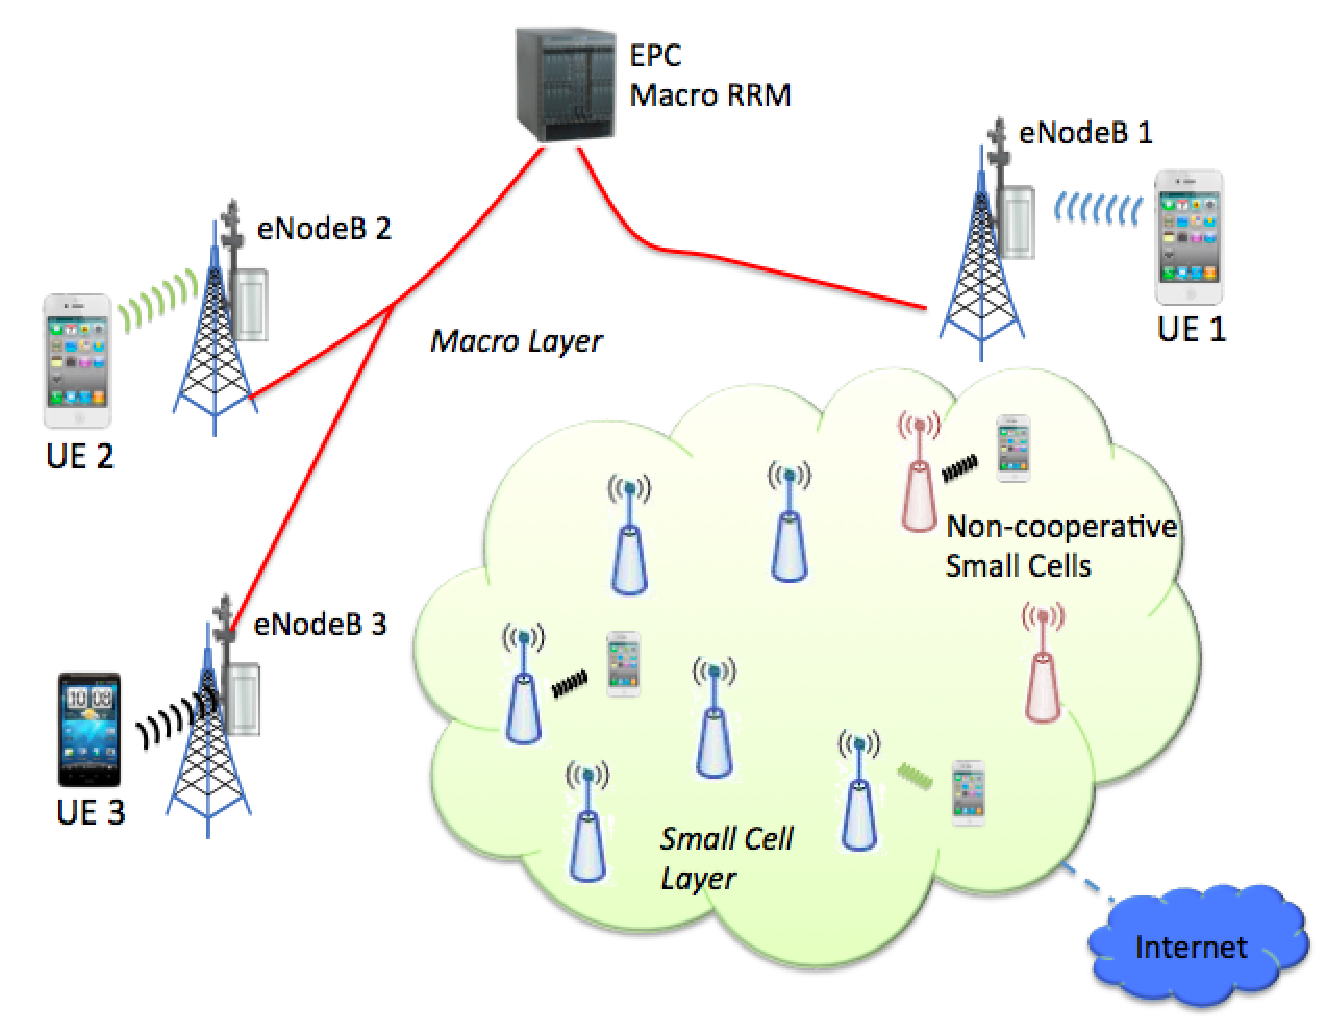
\includegraphics[width=8cm]{gcimages/architecture}
    \caption{Архитектура сети: макро уровень и уровень малых сот (кооперативные и некооперативные)}
    \label{fig:architecture}
\end{figure}

Рис.~\ref{fig:architecture} иллюстрирует типичный сценарий развертывания гетерогенных сетей~\cite{6824744}, которые обычно встречаются на практике. Они состоят из следующих элементов:

\begin{itemize}
\item[$\cdot$] Базовые макро станции (или eNodeB), которые используются для обеспечения основного покрытия сотовой сети. Базовые станции обычно конфигурируются по заранее подготовленным схемам, полученной на предварительном этапе радио-планирования. Качество покрытия базовых макро станций обычно ухудшается на границах соты и в помещениях из-за потерь сигнала и многолучевого замирания. 
\item[$\cdot$] Малые соты (HeNBs) - базовые станции малой дальности, которые в основном развернуты внутри помещений. Малые соты преимущественно развертываются без предварительного согласования и эксплуатируются без контроля со стороны оператора.
\item[$\cdot$] Некооперирующие соты - отдельный класс сетевых элементов, статически настроенные сотовым оператором или по какой-то причине действующие в рамках иных наборов правил, нежели рассматриваемые малые соты. В данной работе эти агенты (наряду с другими источниками помех) образуют ''поведение макросреды''.
\item[$\cdot$] Абонентское оборудование (UEs) - здесь мы не делаем различий между пользователями макросот и малых сот. Мы предполагаем, что пользователя всегда обслуживают базовая станция с самым сильным сигналом (что в большинстве случаев является верным предположением на практике)
\item[$\cdot$] Транспортная инфраструктура: базовые макро станции подключаются к пакетному ядру оператора (ЕРС) через выделенную линию, тогда как малые соты соединены через интернет. Отстутсвие прямой связи между ними делает распределенное алгоритмы управления более практичным для таких систем.
\end{itemize}

\subsection{Системные требования}
В этой главе мы предъявляем следующие требования:
\begin{enumerate}
\item алгоритм должен адаптироваться к различным схемам развертывания, условиям макросреды и типам трафика~\cite{TS36.300}.
\item управление системой должно происходить без вмешательства или предварительной конфигурации (требование самоорганизации)~\cite{TS36.902}.
\item отсутствие связи с посторонними агентами, чтобы избежать проблем с качеством транспортной сети и несовместимостью с проприетарными интерфейсами.
\item скорость сходимости алгоритма должна быть сопоставима с типичной скоростью изменений в системе.
\end{enumerate}

\section{Исследование структуры целевой функции}

\subsection{Модель системы}
Мы рассматриваем систему осуществляющую передачу пользовательских данных в нисходящем канале с использованием технологии мультиплексирования с ортогональным частотным разделением каналов (OFDMA)~\cite{4534773}. Система состоит из $I$ примыкающих друг к другу базовых станций и $K$ активных пользователей (абонентских устройств). Пусть $\mathcal{I} = \{1, 2, ..., I\}$ обозначает множество базовых станций, и $\mathcal{K} = \{1, 2, ..., K\}$. Дополнительно обозначим количество пользователей, обслуживаемых базовой станцией $i$ как $K(i)$. Таким образом, $K = \sum_{i=1}^L{K(i)}$.

Множество ресурсных блоков, доступных каждой базовой станции обозначим как $\mathcal{N} = \{1,2,...,N\}$. В технологии OFDMA доступный радиоспектр разделяется на несколько каналов, где каждый из каналов состоит из последовательных ортогональных OFDM-поднесущих. Ресурсный блок (РБ) представляет собой минимальную единицу, доступную для планирования передачи данных пользователям. Он состоит из 12 последовательных поднесущих в частотной области и 7 OFDM-символов с циклическим преффиксом во временной области (6 символов для расширенного преффикса).~\cite{tichv} Ресурсы выделяются и распределяются между пользователями базовой станции каждую миллисекунду (TTI = 1мс, Transmit Time Interval).

Когда при выделении ресурсов используется простая Reuse-1 модель,  каждому ресурсному блоку сопоставляется одинаковая мощность передачи $\frac{P_{max}}{N}$,  где $P_{max}$ есть максимальная мощность передачи базовой станции в  нисходящем канале. Соотношение сигнал/шум для пользователя $k$,  подключенного к базовой станции $I$ и обслуживаемого в ресурсном блоке $n$ задается следующим выражением~(\ref{eq:sinr}):

\begin{equation}
    \label{eq:sinr}
    \sigma_{k,i,n} = \frac{\pi_{i,n} G_{k,i,n}}{N_0 + \sum_{i'\neq i}{\pi_{i',n} G_{k,i',n}}}
\end{equation}
, где $\pi_{i,n}$ - мощность передачи базовой станции $i$ в ресурсном блоке $n$, $G_{k,i,n}$ - коэффициент усиления (ослабления) канала между базовой станцией $i$ и пользовательским устройством $k$, обслуживаемым в ресурсном блоке $n$ и $N_0$ - мощность теплового шума. Индексы $i$ и $i'$ относятся к полезному и интерферирующим сигналам соответственно. Для удобства список используемых обозначений собран в таблице~\ref{tbl:notations}.


\begin{table} [htbp]
  \label{tbl:notations}
  \centering
  %\captionsetup{width=15cm}
  \caption{Используемые обозначения}\label{Ts0Sib}%
  \begin{tabular}{| p{1cm} || p{10cm} |}
  \hline
  \hline
  \centering $i$ &  Индекс базовой станции   						\\
  \centering $k$ &  Индекс пользовательского устройства     		\\
  \centering $n$ &  Индекс ресурсного блока   						\\
  \centering $\mathcal{I}$ & Множество базовых станций				\\
  \centering $\mathcal{K}$ & Множество пользовательских устройств	\\
  \centering $\mathcal{K}(i)$ & Множество пользовательских устройств, ассоциированных с базовой станцией $i$\\
  \centering $\mathcal{N}$ & Множество ресурсных блоков\\
  \centering $\rho_{k,i,n}$ & Пропускная способность пользователя $k$, обслуживаемого в ресурсном блоке $n$ базовой станции $i$\\
  \centering $\pi_{i,n}$ & Мощность передачи базовой станции $i$ в ресурсном блоке $n$\\
  \centering $G_{k,i,n}$ & Коэффициент усиления (ослабления) канала между базовой станцией $i$ и пользовательским устройством $k$\\
  \centering $N_0$ & Мощность теплового шума\\
  \centering $\theta_{k,n}$ & Процент времени, занимаемый пользователем $k$ в ресурсном блоке $n$ \\
  \centering $\sigma_{k,i,n}$ & Соотношение сигнал/шум для пользователя $k$, обслуживаемого в ресурсном блоке $n$ базовой станции $i$ \\
  \centering $P_{max}$ &  Максимальная мощность передачи базовой станции в  нисходящем канале\\
  \centering $\pi_{min}$ & Минимальная мощность передачи в ресурсном блоке \\
  \centering $\mathcal{I}'(i)$ & Множество базовых станций смежных с $i$\\
  \hline
  \hline
  \end{tabular}
\end{table}

\subsection{Постановка оптимизационной задачи}
В данном разделе ставится цель максимизировать суммарную пропускную способность сети базовых станций с обеспечением честности распределения ресурсов между пользователями за счет управления мощностью передачи в реcурсных блоков. Пиковая пропускная способность пользователя $k$, обслуживаемого в ресурсном блоке $n$ базовой станции $i$ задается следующим образом:

\begin{equation}
    \label{eq:throughput}
    \rho_{k,i,n} = \log \left(1 + \frac{\pi_{i,n} G_{k,i,n}}{N_0 + \sum_{i'\neq i}{\pi_{i',n} G_{k,i',n}}}\right)
\end{equation}

Обозначим за $\theta_{k,n}$ процент времени, занимаемый пользователем $k$ в ресурсном блоке $n$. Таким образом, средняя пропускная способность для пользователя задается следующим выражением~(\ref{eq:uthroughput}):

\begin{equation}
    \label{eq:uthroughput}
    \sum_{n \in \mathcal{N}} \theta_{k,n} \cdot \rho_{k,i,n}
\end{equation}

Задачу оптимизации для рассматриваемого сценария можно сформулировать следующим образом. Целевая функция $\eta(\pi, \theta)$ состоит из суммы логарифмов показателей пропускной способности для обслуживаемых пользователей.

\begin{equation}
\label{eq:maximize}
\eta = \sum_{i \in \mathcal{I}} \sum_{k \in \mathcal{K}(i)} \log \left(\sum_{n \in \mathcal{N}} \theta_{k,n} \cdot \log \left(1 + \frac{\pi_{i,n} G_{k,i,n}}{N_0 + \sum_{i'\neq i}{\pi_{i',n} G_{k,i',n}}}\right)\right) 
\end{equation}

Такая структура целевой функции $\sum_{k=1}^K \log(r_k)$ (см.~(\ref{eq:maximize})) традиционно используется для максимизации суммарной пропускной способности в системах с $K$ пользователями для достижения справедливости распределения ресурсов. Может быть показано, что для решения $r^* = (r_1,r_2,...,r_K), r^* \in \Lambda$ задачи максимизации справедливо  неравенство (\ref{eq:propfairness}),  совпадающее с определением \textit{пропорционально справедливого} распределения ресурсов между $K$ пользователями~\cite{ETT:ETT4460080106}.

\begin{equation}
\label{eq:propfairness}
\sum_{k=1}^K \frac{r_k - r_k^*}{r_k^*} \leq 0, \forall r \in \Lambda
\end{equation}

Задача максимизации фукционала $\eta$ дополняется следующими ограничениями: выражения~(\ref{eq:limitationsa})--(\ref{eq:limitationsc}) гарантируют, что ресурсный блок не используется повторно сразу несколькими пользователями одной базовой станции,  ограничения~(\ref{eq:limitationsd})~и~(\ref{eq:limitationse}) соответствуют физическим ограничениям на суммарную мощность передачи по всем ресурсным блокам и минимальной мощности передачи в отдельном ресурсном блоке.

\begin{subequations}
\begin{equation}
\label{eq:limitationsa}
\sum_{k \in \mathcal{K}(i)} \theta_{k,n} \leq 1, \forall n \in \mathcal{N}
\end{equation}

\begin{equation}
\label{eq:limitationsb}
\sum_{n \in \mathcal{N}} \theta_{k,n} \leq 1, \forall k \in \mathcal{K}(i) 
\end{equation}

\begin{equation}
\label{eq:limitationsc}
0 \leq \theta_{k,n} \leq 1, \forall k \in \mathcal{K}(i), \forall n \in \mathcal{N}
\end{equation}

\begin{equation}
\label{eq:limitationsd}
\sum_{n \in \mathcal{N}} \pi_{i,n} \leq P_{max}, \forall i \in \mathcal{I}
\end{equation}

\begin{equation}
\label{eq:limitationse}
\pi_{i,n} \geq \pi_{min}, \forall i \in \mathcal{I}, \forall n \in \mathcal{N}
\end{equation}
\end{subequations}

\subsection{Декомпозиция оптимизационной задачи}
Для упрощения задачу максимизации фукционала~(\ref{eq:maximize}) возможно разделить на две независимые задачи оптимизации - задачу распределения ресурсов между пользователями и задачу управления мощностью в ресурсных блоках. Воспользуемся неравенством для выпуклой функции ($f\left(\sum _{{i=1}}^{{n}}q_{i}x_{i}\right)\leq \sum _{{i=1}}^{{n}}q_{i}f(x_{i})$), чтобы получить нижнюю оценку для целевой функции $\eta$:

\begin{equation}
    \label{eq:jensen}
    \log{\sum_{n \in \mathcal{N}} \theta_{k,n} \cdot \rho_{k,i,n}} \geq \frac{\sum_{n \in \mathcal{N}} \log{\theta_{k,n} \cdot \rho_{k,i,n}}}{|\mathcal{N}|} + \log{|\mathcal{N}|}
\end{equation}

Таким образом для получения нижней оценки максимума функции $\eta(\pi, \theta)$ (см. формулу ~(\ref{eq:maximize})) предлагается производить оптимизацию функционала $\eta'$ с ограничениями ~(\ref{eq:limitationsa})--(\ref{eq:limitationse}). В такой постановке задачу оптимизации возможно разделить на две независимые задачи - задачу распределения ресурсов между пользователями и задачу управления мощностью в ресурсных блоках.

\begin{equation}
\label{eq:maximizealt}
\eta' = \sum_{i \in \mathcal{I}} \sum_{k \in \mathcal{K}(i)} \sum_{n \in \mathcal{N}} (\log(\theta_{k,n}) + \log( \rho_{k,i,n}))
\end{equation}

\section{Схема управления на основе обучения с подкреплением}
\begin{figure}
    \centering
    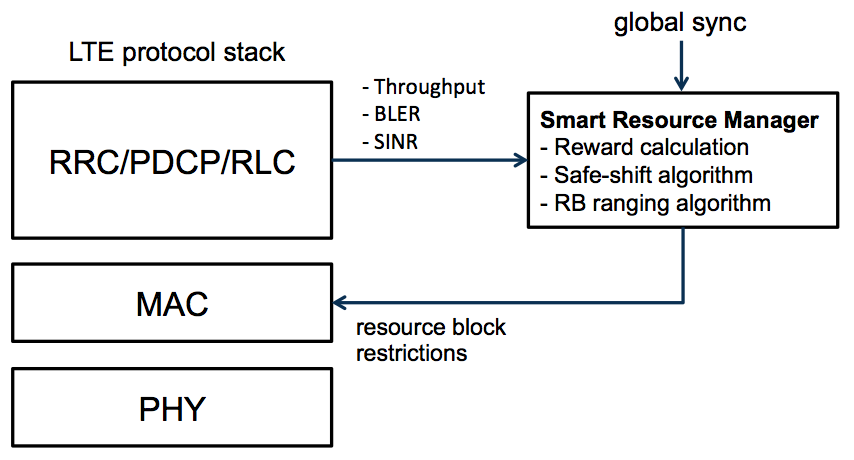
\includegraphics[width=8cm]{gcimages/algo_arch}
    \caption{Структура алгоритма и место в стеке протоколов LTE: PHY - физический уровень, MAC - уровень управления доступом к среде, RRC/PDCP/RLC - верхние уровни стека LTE}
    \label{fig:algo_arch}
\end{figure}

На Рис.~\ref{fig:algo_arch} представлена упрощенная структура алгоритма в стеке протоколов сети LTE. Можно заметить, что входящие или исходящие каналы управления не используются. Таким образом предлагаемое решение не налагает каких-либо требований на качество канала между базовыми станциями и выполняется локально на каждой малой соте.
Общий принцип алгоритма заключается в следующем. Основываясь на статистике производительности слоя L2~\cite{TS36.300} (например, BLER, спектральная эффективность) каждая малая сота локально принимает решение об использовании ресурсных блоков на последующем периоде времени. Единственный внешний входящий канал управления - глобальный источник точного времени. Он используется для выполнения синхронных операций (безопасный сдвиг) в пределах группы малых сот. После принятия решения о распределении ресурсов в каждой соте, выбранные ресурсные блоки  распределяются между пользователями базовой станции на уровне доступа к среде.

\subsection{Схема распределения радиоресурсов}
В этой части мы рассмотриваем разнородные сети LTE состоящие из множества малых сот, сосуществующих с окружающими базовыми макро станциями. Базовые макро станции и малые соты работают в одном частотном диапазоне, чтобы увеличить повторное использование пространственной частоты.

Для координации интерференции между соседними сотами каждая малая сота автономно принимает решения о распределении частот. Весь доступный частотный диапазон разбивается на ряд поддиапазонов $b_{j}$, где $j=1, .., N$ и $N$ - общее количество поддиапазонов. Распределение ресурсов внутри каждой базовой станции осуществляется планировщиком с алгоритмом пропорционального справедливого разделения (Proportional fair).

В момент времени $t$ автономный агент должен решить, какой поддиапазон $b(t+1)$ из имеющегося спектра доступен для использования на следующем временном промежутке $t+1$. Мы предлагаем схему обучения, состоящую из двух уровней (см. Рис.~\ref{fig:algo_arch}):

\begin{itemize}
\item[$\cdot$] параллельное обучение с подкреплением~\cite{4445757}, с $N\times N$ матрицей перехода $T(t)$. Она определяет вероятность перехода агента из поддиапазона $i$ в поддиапазон $j$ в момент времени $t$. Элементы матрицы периодически обновляются полученными наградами $RW_{ij}(t) = e^{(C_i(t-1) - C_j(t))}$, где $C_j(t)$ - достигаемая пропускная способность или количество пользователей с удовлетворенными требованиями к качеству обслуживания в момент времени $t$ при использовании поддиапазона $j$.
\item[$\cdot$] исследование макросреды (см. разд.~\ref{sec:safe_shift}), верхний уровень алгоритма с исследованием макросреды без вмешательства, где обучаемые агенты синхронно выполняют согласованную смену схемы использования ресурсов (безопасный сдвиг). $RW_{ij}(t_{sh})$ рассчитывается точно так же, как $RW_{ij}(t)$, но во время этапа безопасного сдвига. Этот шаг отвечает за обеспечение сосуществования с невзаимодействующими агентами и исследования макросреды.
\end{itemize}

Матрица перехода $T$ определяет вероятность перехода из поддиапазона $i$ к поддиапазону $j$. Значения $T_{ij}(t)$ и $T_{ij}(t_{sh})$ обновляются на каждой итерации (каждую 1 мс) на основе функции вознаграждения как описано в~(\ref{eq:tm_update}).
\begin{equation}
    \label{eq:tm_update}
    T_{ij}(t) = (1-\alpha-\beta)T_{ij}(t-1) + \alpha RW_{ij}(t) + \beta RW_{ij}(t_{sh})
\end{equation}
\begin{equation}
    \label{eq:tm_update_c}
    RW_{ij}(t) = e^{(C_i(t-1) - C_j(t))}
\end{equation}
где:

\begin{itemize}
\item[$\cdot$]$ \alpha$ - коэффициент обучения, определяющий скорость сходимости алгоритма и соотношение этапов исследования и эксплуатации. Оптимальное значение для этого параметра подбирается экспериментально в ходе симуляций.
\item[$\cdot$] $\beta$ - коэффициент обучения ($\beta < \alpha$) для макросреды, определяющий скорость сходимости алгоритма верхнего уровня.
\end{itemize} 

В то время как соты не имеют одинаковых знаний об уровне занятости/интерференции каждого поддиапазона, матрица перехода $T$ обновляется независимо для каждой соты. В определенной степени, это может привести к уменьшению скорости сходимости алгоритма. Моделирование показывает, что этим поведением можно эффективно управлять с помощью тонкой настройки коэффициентов обучения. В следующем разделе предложен дополнительный метод для повышения скорости сходимости алгоритма.

\subsection{Исследование макросреды: алгоритм безопасного сдвига}
\label{sec:safe_shift}
Любой агент в каждый момент времени наблюдает ответ окружающей среды $\gamma = \gamma^{CL} + \gamma^{ML}$, который состоит из двух частей: $\gamma^{CL}$ - компонент, определяемый поведением соседних агентов, а $\gamma^{ML}$ - независимый компонент, определяемый слоем макросреды.
Рисунок~\ref{fig:channel_exploration_blocked} иллюстрирует простой случай так называемой блокировки канала, где этап исследования окружающей среды $\gamma^{ML}$ агентом №2 заблокирован компонентой $\gamma^{CL}$, обусловленной выбором диапазона агента №1. Аналогичным образом на практике подавляющее большинство попыток разведки будут заблокированы ответом канала $\gamma_b^{CL}$ соседей. 

\begin{figure}
    \centering
    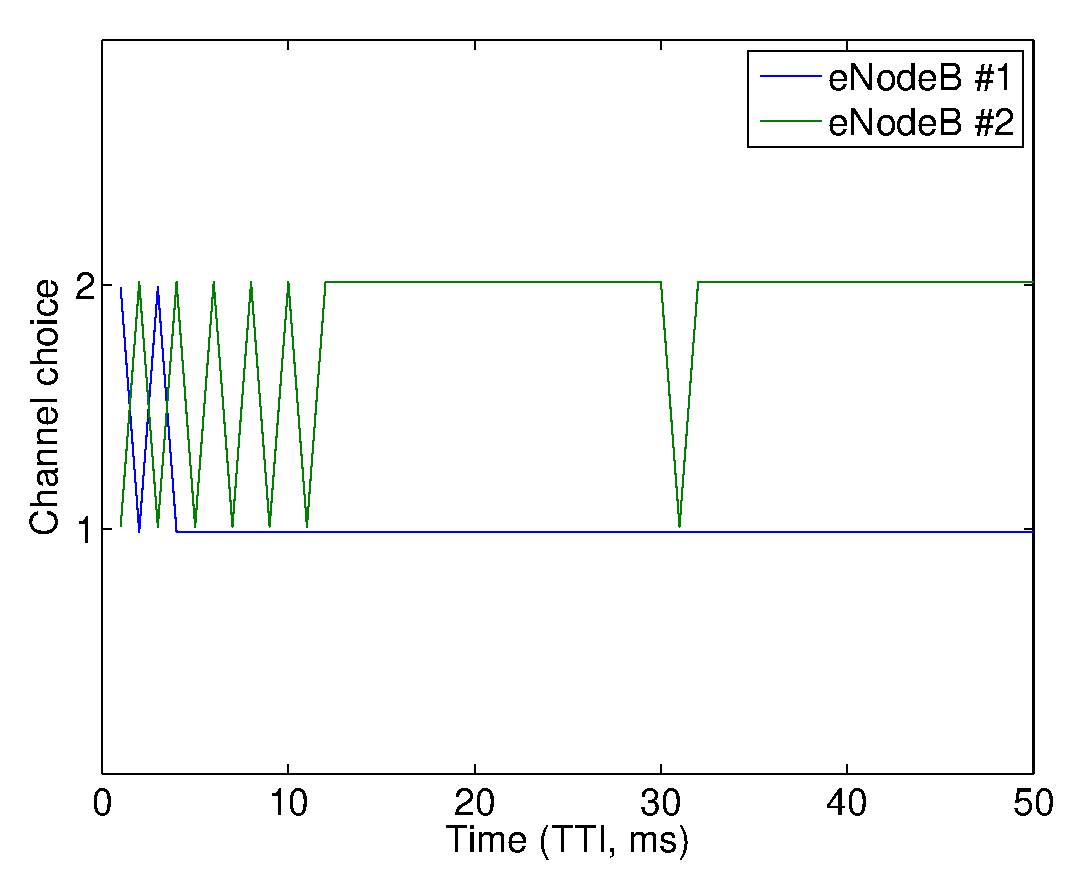
\includegraphics[width=8cm]{gcimages/channel_exploration_blocked}
    \caption{Пример эффекта блокировки канала. Оба частотных диапазона заблокированы.}
    \label{fig:channel_exploration_blocked}
\end{figure}

Чтобы побороть описанный эффект мы заставляем каждого агента изучать ответ макросреды $\gamma_b^{ML}$ в пределах каждого параллельного этапа обучения $t$ - процедуры безопасного сдвига. В рамках этой процедуры каждый агент последовательно изучает поддиапазоны в следующем порядке: ${(b_{t+1}+i)~mod~N}, i=1..N$. Очевидно, что это изменение не повлияет на компонент ответа $\gamma^{CL}$, так как агенты на пересекающихся поддиапазонах в момент времени $t$ по-прежнему используют те же поддиапазоны в момент времени ${t+1}$. В то же время компонент $\gamma^{ML}$ базового ответа окружающей среды изменяется.

Изучая отличия ответов окружающей среды $\gamma_b$, мы можем скорректировать оценки величин $\gamma_b^{ML}$ и $\gamma_b^{CL}$ для каждого агента в отдельности. Чтобы сохранить свойство локальности алгоритма, мы предлагаем управлять моментом запуска процедуры безопасного сдвига для каждого агента при помощи источника глобального времени. Значения функции вознаграждения при процедуре безопасного сдвига учитываются в соответствующей статистике для поддиапазонов в качестве отдельного компонента (см. формулу~\ref{eq:tm_update}). В результате обновления условия $\beta RW_{ij}(t_{sh})$, обучаемые агенты должны выбрать поддиапазоны с лучшим ответом макросреды.

Следующий эксперимент иллюстрирует простой пример процедуры безопасного сдвига. Рассмотрим случай двух малых сот разделяющих два частотных поддиапазона, где один из поддиапазонов занят невзаимодействующим агентом (например, базовая макро станция). После схождения процесса обучения малые соты 1 и 2 используют подздиапазоны 2 и 1 соответственно, каналы блокируются для исследования. Пусть поддиапазон 1 также занимает базовая макро станция или невзаимодействующий агент. Результат влияния процедуры безопасного сдвига на общую пропускную способность сети представлен на рис.~\ref{fig:safe_shift_overal_throughput}, где сдвиги производятся в моменты времени $t_1=200$ мс и $t_2=400$ мс. Этот шаг не влияет на взаимную интерференцию между агентами, но измененяет уровень помех от макросреды. Прирост около $10\%$ достигается без необходимости возобновления параллельного обучения для обоих агентов.

\begin{figure}
    \centering
    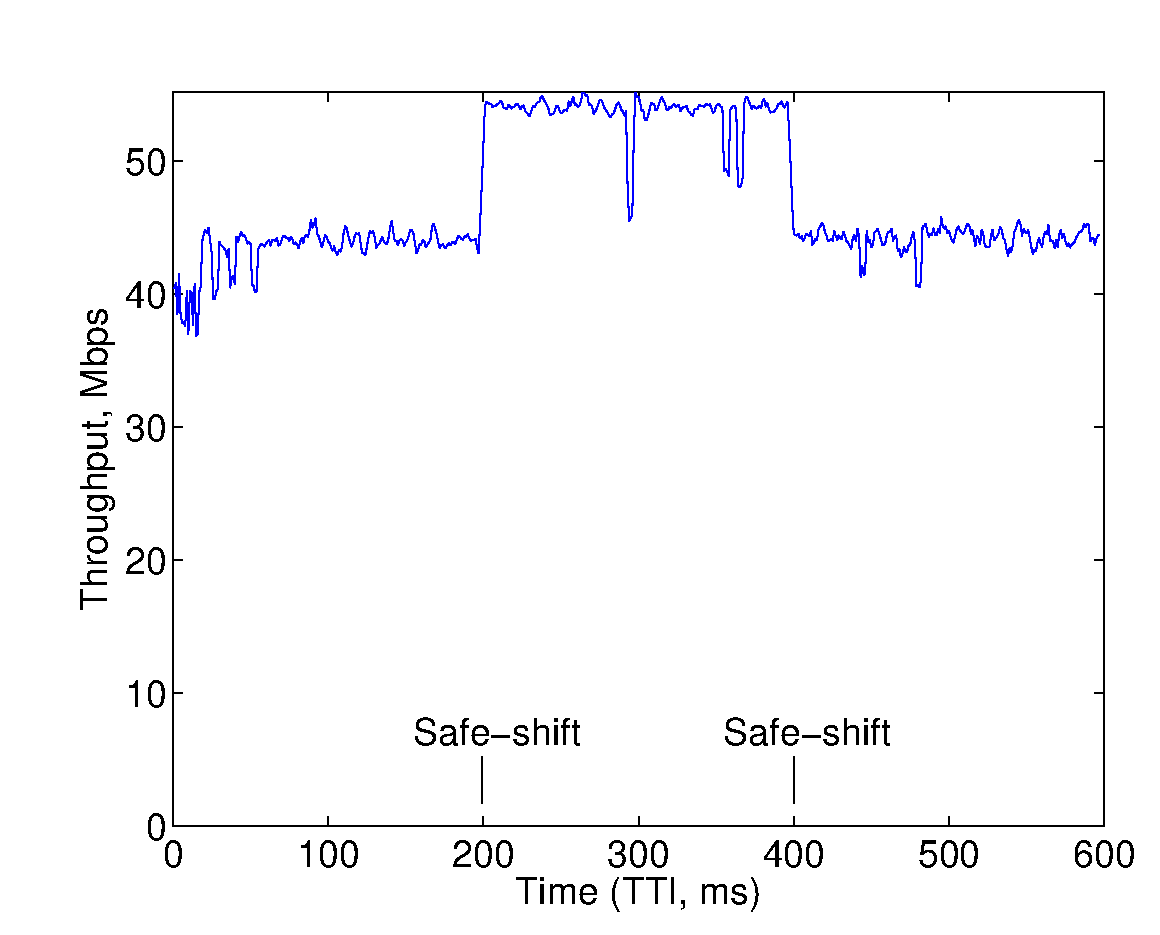
\includegraphics[width=8cm]{gcimages/overal_throughput}
    \caption{Прирост пропускной способности. Процедура безопасного сдвига инициирована в моменты времени $t_1=200$ мс и $t_2=400$ мс }
    \label{fig:safe_shift_overal_throughput}
\end{figure}

\subsection{Исследование скорости сходимости, выкалывание множества состояний}
В процессе обучения агенты постоянно изменяют свое состояние. Это в свою очередь инвалидирует стратегии других агентов, делая исходные условия, на которых они построены, устаревшими. Общий подход к этой проблеме заключается в том, чтобы считать этот эффект частью динамично изменяющейся среды. Однако, это предположение ослабляется в случае параллельного обучения множества агентов, где поведение динамической среды в большей степени определяется самими агентами.
Для того, чтобы преодолеть определяющую роль случайного исследования в структуре окружающей среды, мы предлагаем следующий способ. Идея в том, чтобы предварительно заставить агентов вести себя уникальным образом. В этом случае даже в процессе обучения посредством случайного исследования агенты могли бы получать статистически значимые наблюдения о поведении соседних агентов. Для этого мы предлагаем случайно выколоть часть $p$ $(p< 1)$ элементов матрицы перехода $TM_{ij}$ для каждого агента. Ожидается, что этот метод значительно уменьшит время сходимости процесса обучения.


\begin{figure}
    \centering
    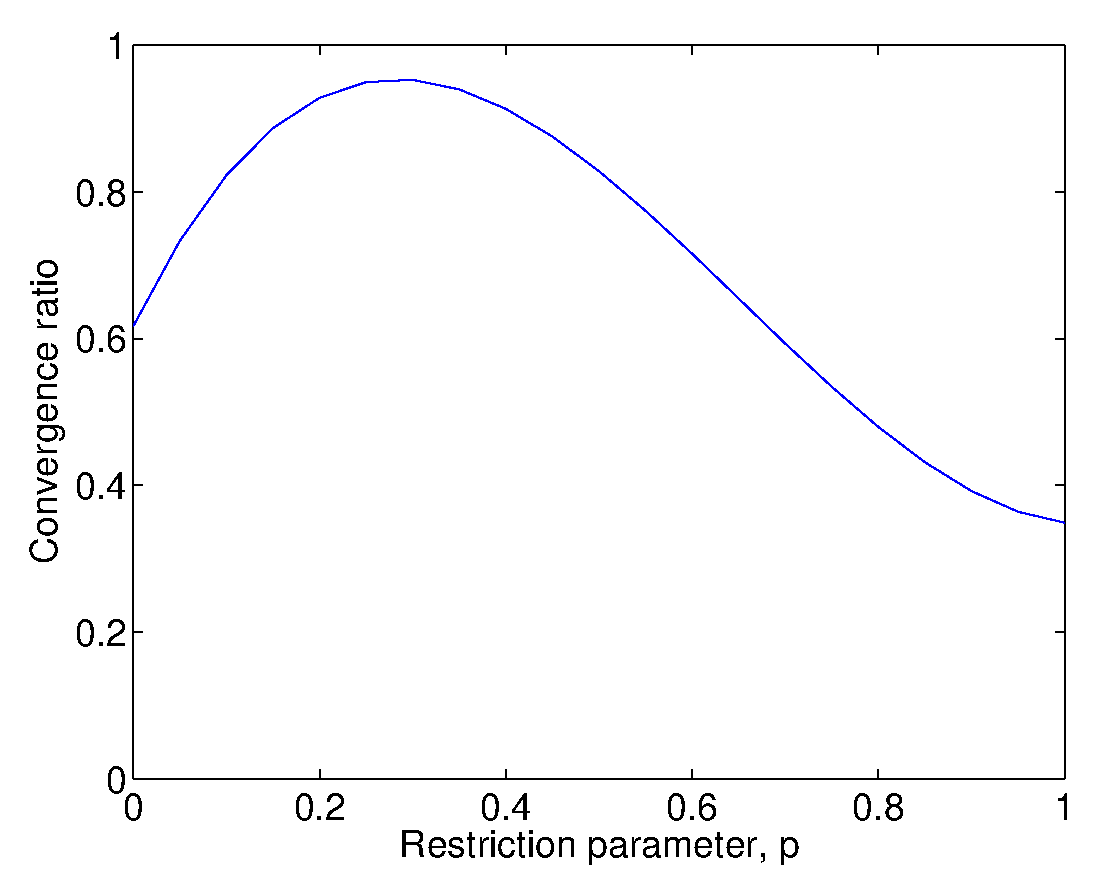
\includegraphics[width=8cm]{gcimages/restrict_p_sm}
    \caption{Средняя скорость сходимости в зависимости от параметра $p$ (тренд)}
    \label{fig:restrict_profit}
\end{figure}

На рисунке~\ref{fig:restrict_profit} проиллюстрировано поведение значения скорости сходимости в зависимости от параметра $p$ (показания усредненны для случайного набора из 500 прогонов иммитационной модели). Под скоростью сходимости понимается отношение продолжительности этапа эксплуатации к общей продолжительности работы системы. Значение $p = 0$ соответствует случаю, когда на переходные правила не накладывается никаких ограничений. Значение $p>0$ - конфигурации, когда некоторая часть переходов случайным образом запрещена для каждого агента. Видно, что для определенного значения ($p=0.3$) коэффициент сходимости увеличивается на $20\%$.

% \subsection{Channel blocking}

\section{Оценка эффективности}

Для анализа производительности, мы проводим моделирование с помощью симулятора, основанном на программном продукте Vienna LTE-A Downlink System Level Simulator (\cite{VTC2010}). Сеть состоит из 2-х уровней - группа малых сот (находящихся внутри помещения) соседствует с базовой макро станцией. Малые соты располагаются в ячейках 5х5 сетки по правилам, указанным в рекомендации консорциума 3GPP ~\cite{R4-092042}. Пользователи равномерно распределены внутри помещения. Предполагается, что каждый пользователь обслуживается базовой станцией с самым сильным сигналом. Рассматриваемые модели распространения сигнала и замирания в канале основаны на рекомендациях ~\cite{R4-092042}. Основные параметры модели, используемые по-умолчанию приведены в таблице~\ref{table:simulation_parameters}.

На рисунке~\ref{fig:fcdf3} показана интегральная функция распределения пропускной способности пользователей для множества прогонов моделирования. Предложенный алгоритм сравнивается с алгоритмом обучения, описанным в~\cite{mab}, где базовые станции принимают решения о распределении поддиапазонов с учетом занятости ресурсов каждой из окружающих сот. Видно, что предлагаемый механизм безопасного сдвига способен увеличить среднюю емкость сети на $8 - 10\%$ без негативного воздействия на честность распределения ресурсов.

\begin{table}
\centering
    \caption{Параметры моделирования}
    \begin{tabular}{|l l|} 
    \hline
    \textbf{Параметр} & \textbf{Описание} \\
    \hline
    \multicolumn{2}{|c|}{\textbf{Детали сценария}} \\
    \hline
    Основой сценарий & 5x5 Grid~\cite{R4-092042} \\
    \hline
    Выходная мощность & 23 дБм \\
    \hline
    Количество базовых станций & 7 \\
    \hline
    Количество пользователей & 28 \\
    \hline
    Планировщик & PF \\
    \hline
    Трафик & BE \\
    \hline
    Тип антенн & Всенаправленные \\
    \hline
    Ширина канала & 20 МГц \\
    \hline
    Продолжительность TTI  & 1 мс \\
    \hline
    Продолжительность симуляции & 300 TTI, 1 ч \\
    \hline
    \multicolumn{2}{|c|}{\textbf{Модель канала}} \\
    \hline
    Несущая частоты & Band 7 \\
    \hline
    Плотность мощности теплового шума  & -174 дБм/Гц \\
    \hline
    Затенение канала & Log-normal, 8 дБ \\
    \hline
    Замирание канала & Плоское замирание \\
    \hline
    \multicolumn{2}{|c|}{\textbf{Параметры алгоритма}} \\
    \hline
    $\alpha$ & 0.1 \\
    \hline
    $\beta$ & 0.05 \\
    \hline
    Коэффициент выкалывания, $p$ & 0.3 \\
    \hline
    \end{tabular}
    \label{table:simulation_parameters}
\end{table}

Эффективность предложенного алгоритма сравненивается с традиционной статической схемой разбиения полосы частот (см., например, \cite{4907410}): 

\textbf{Алгоритм Reuse 1}: каждая базовая станция использует всю доступную полосу пропускания (20 МГц, см. таблицу~\ref{table:simulation_parameters}). Затем ресурсы распределяются между пользователями с помощью пропорционального справедливого планировщика.

\textbf{Алгоритм Reuse 3}: каждой базовой станции выделяется треть всего доступного диапазона. Поддиапазонное распределение настроено так, что соседние базовые станции не используют перекрывающиеся поддиапазоны.

\begin{figure}
    \centering
    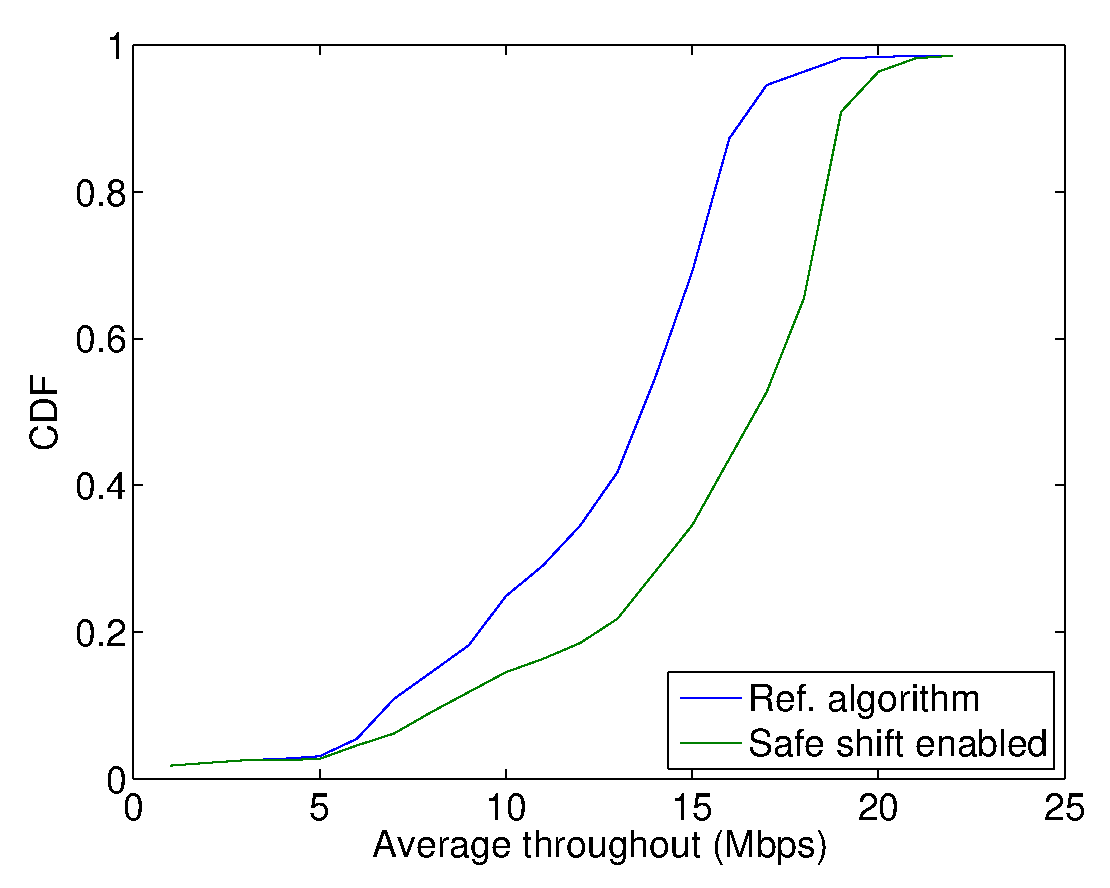
\includegraphics[width=8cm]{gcimages/fcdf3}
    \caption{Функция распределения пропускной способности для пользователей. Алгоритм безопасного сдвига}
    \label{fig:fcdf3}
\end{figure}

На рисунке ~\ref{fig:scdf} показана интегральная функция распределения соотношений сигнал-шум (SINR) для пользователей при использовании предлагаемого алгоритма разделения ресурсов. Значение SINR (соотношения сигнала к интерференции и шуму) рассчитывается для каждого пользователя после выделения ресурсных блоков.
\begin{equation}
    \label{eq:SINR}
    {SINR}_u(b) = \frac{P_u(b) G_u}{\sum_{i \in \eta} P_i(b) G_{u,i} + \sigma^2}
\end{equation}
где $P_u(b)$ - мощность передачи в ресурсном блоке $b$ при обслуживании пользователя $u$; $G_{u,i}$ - ослабление канала между пользователем $u$ и базовой станцией $i$; и $\eta$ - множество соседних базовых станций. Обратим внимание, что $P_i(b) = 0$, если базовая станция $i$ не обслуживает пользователей в поддиапазоне $b$.

\begin{figure}
    \centering
    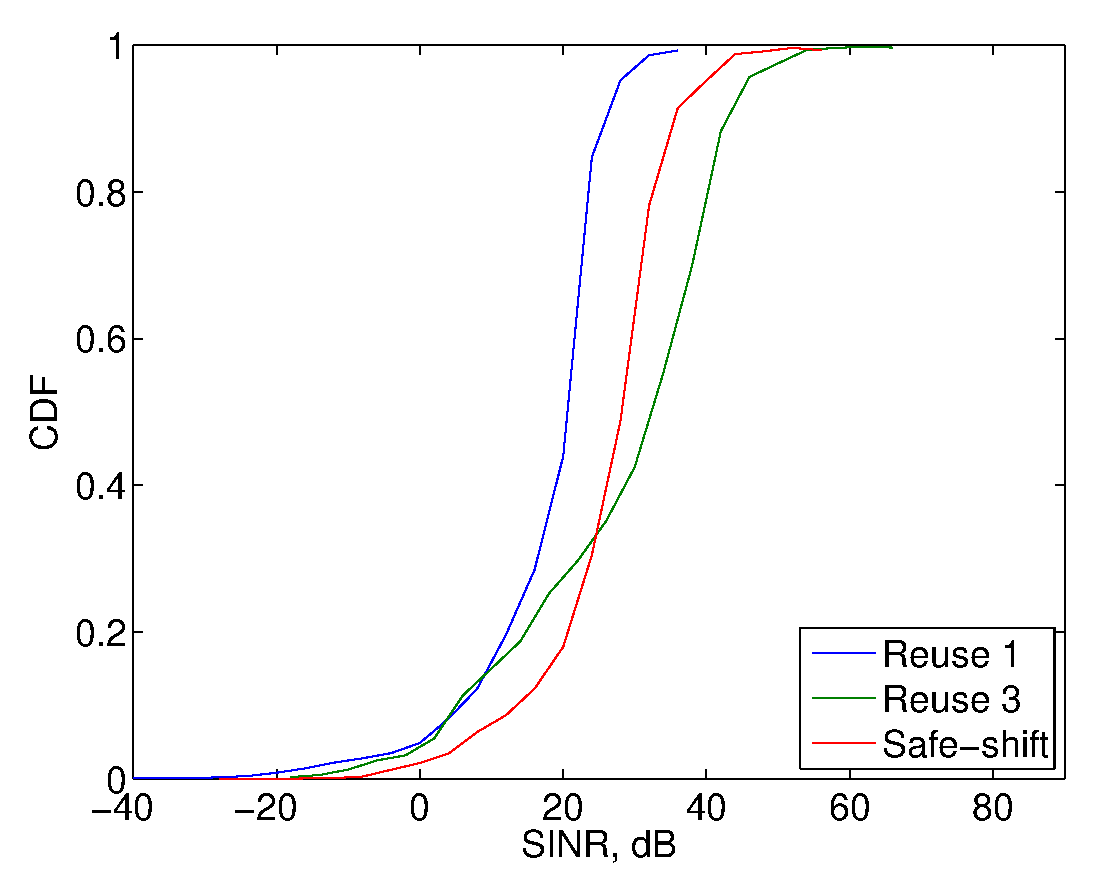
\includegraphics[width=8cm]{gcimages/scdf}
    \caption{Функция распределения соотношений сигнал-шум (SINR) для пользователей сети}
    \label{fig:scdf}
\end{figure}

Из рисунка~\ref{fig:scdf} можно заключить, что предложенный алгоритм способен самостоятельно найти оптимальную схему распределения поддиапазонов и превосходит традиционные централизованные статические схемы разделения ресурсов. Мы также отмечаем, что процедура безопасного сдвига позволяет осуществить исследование без вмешательства в ранее установленную схему распределения ресуров. Это позволяет системе сходится к более выгодной конфигурации без дополнительных затрат, связанных с автономным исследованием. Показано, что предлагаемая процедура позволяет сократить количество шагов случайного исследования среды на $20\%$, при этом оставаясь выше по эффективности на этапе эксплуатации, чем базовый алгоритм.

\section{Обсуждение}
В этой главе мы представили механизм распределения радиоресурсов для координации интерференций между соседними сотами в плотной гетерогенной сети. Он распределяет ресурсы системы на основе мультиагентного параллельного алгоритма обучения. Основной упор делается на сосуществование малых сотовых систем с невзаимодействующей макросредой. Мы также предложили прием для повышения эффективности параллельного обучения за счет снижения эффекта блокировки исследования внешней среды. Воспользовавшись так называемой процедурой безопасного сдвига, мы продемонстрировали способ повышения общей эффективности обучения и обеспечения сосуществования с окружающей средой в многоагентной среде.

Данный алгоритм предполагает гибкий механизм для контроля скорости сходимости в случае разделения радиоресурса на несколько поддиапазонов. В качестве входных данных для алгоритма, мы используем стандартные метрики 3GPP, доступные локально на любой коммерческой малой соте, что делает его легко реализуемым на практике. Вычислительная сложность алгоритма невысока всвязи с итеративным характером получения итогового решения.

Моделирование на системном уровне доказало эффективность предложенного решения в условиях реалистичных сценариев развертывания, рекомендованных консорциумом 3GPP. В нашем исследовании мы показали, что предложенный алгоритм работает в различных разнородных сценариях и превосходит эталонные алгоритмы без негативного влияния на скорость сходимости. Дальнейшие исследования направлены на развитие усовершенствованного алгоритма, способного динамически регулировать размеры поддиапазонов.
